\def\mySecNum{12.3}
\mySection{\mySecNum~Option Greeks}
%-------------- start slide -------------------------------%{{{ 1 Intro
\begin{frame}[fragile,t]
	\frametitle{What happens to the option price\\ when one and only one input changes?}

\begin{itemize}
	\item Delta ($\Delta$): change in option price when stock price increases by \$1
	\item Gamma ($\Gamma$): change in delta when option price increases by \$1
	\item Vega: change in option price when volatility increases by 1\%
	\item Theta ($\theta$): change in option price when time to maturity decreases by 1 day
	\item Rho ($\rho$): change in option price when interest rate increases by 1\%
	\item Psi ($\psi$): change in the option premium due to a change in the dividend yield
		\bigskip
		\mySeparateLine
		\bigskip
	\item The \textcolor{magenta}{Greek measure of a portfolio} is weighted average of Greeks of individual portfolio components
		\begin{equation*}
			\Delta_{\text{portfolio}} =\sum_{i=1}^{N} n_i \Delta_i
		\end{equation*}
\end{itemize}
\end{frame}
%-------------- end slide -------------------------------%}}}
%-------------- start slide -------------------------------%{{{ 1
\begin{frame}[fragile]
\begin{center}
	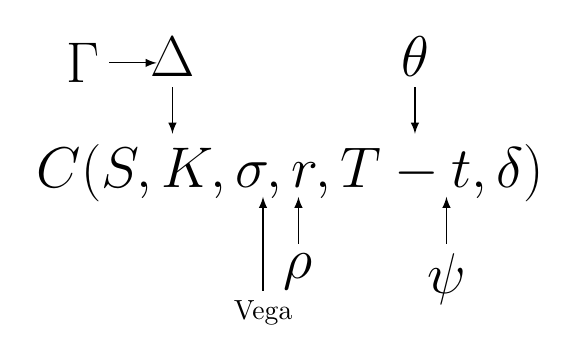
\begin{tikzpicture}[scale=1, transform shape]
		\tikzset{>=latex}
		\node[] (a) at (0,0) {\huge $C(S, K, \sigma, r, T-t,\delta)$};
		\def\len{0.6}
		\draw [<-] (-1.5,0.5) -- ++ (0,\len) node [above] {\huge $\Delta$};
		\draw [<-] (-1.7,0.5+\len+0.3) -- ++ (-\len,0) node [left] {\huge $\Gamma$};
		\draw [<-] (-0.35,-0.3) -- ++ (0,-\len-\len) node [below] {Vega};
		\draw [<-] (0.1,-0.3) -- ++ (0,-\len) node [below] {\huge $\rho$};
		\draw [<-] (1.58,0.5) -- ++ (0,\len) node [above] {\huge $\theta$};
		\draw [<-] (1.98,-0.3) -- ++ (0,-\len) node [below] {\huge $\psi$};
	\end{tikzpicture}
\end{center}
\end{frame}
%-------------- end slide -------------------------------%}}}
%-------------- start slide -------------------------------%{{{ 1 Delta
\begin{frame}[fragile]
	\frametitle{Delta}
	\centering

	\textcolor{magenta}{Delta ($\Delta$)}: change in option price when stock price increases by \$1.
	\bigskip

	\begin{equation*}
		\Delta =
		\begin{cases}
			\displaystyle \frac{\partial C(S,K,\sigma,T-t,\delta)}{\partial S} = +e^{-\delta(T-t)} N(+d_1) & \text{Call} \\[1em]
			\displaystyle \frac{\partial P(S,K,\sigma,T-t,\delta)}{\partial S} = -e^{-\delta(T-t)} N(-d_1) & \text{Put}  \\
		\end{cases}
	\end{equation*}
\end{frame}
%-------------- end slide -------------------------------%}}}
%-------------- start slide -------------------------------%{{{ 1 Proof of Delta
\begin{frame}[fragile,t]
\begin{myexample}
	Demonstrate that
	\begin{equation*}
		\Delta =
		\begin{cases}
			\displaystyle \frac{\partial C(S,K,\sigma,T-t,\delta)}{\partial S} = +e^{-\delta(T-t)} N(+d_1) & \text{Call} \\[1em]
			\displaystyle \frac{\partial P(S,K,\sigma,T-t,\delta)}{\partial S} = -e^{-\delta(T-t)} N(-d_1) & \text{Put}.
		\end{cases}
	\end{equation*}
\end{myexample}
\begin{mysol}
	We only show the call part. By the chain rule:
	\begin{align*}
		\frac{\partial C}{\partial S} = & \quad e^{-\delta (T-t)} N(d_1) \\
                                    & + S e^{-\delta (T-t)} N'(d_1) \frac{\partial d_1}{\partial S} - K e^{-r (T-t)} N'(d_2) \frac{\partial d_2}{\partial S}.
	\end{align*}
	Because $d_2 = d_1 - \sigma \sqrt{T-t}$, we see that
	\begin{align*}
		\frac{\partial d_1}{\partial S} = \frac{\partial d_2}{\partial S}.
	\end{align*}
	It suffices to prove that
	\begin{align*}
		Se^{\delta (T-t)} N'(d_1) = K e^{-r (T-t)} N'(d_2).
	\end{align*}
\end{mysol}
\end{frame}
%-------------- end slide -------------------------------%}}}
%-------------- start slide -------------------------------%{{{ 1 Proof continued
\begin{frame}[fragile,t]
\begin{mysol}( Continued )
	Notice that
	\begin{align*}
		N'(d) = \frac{1}{\sqrt{2\pi}} e^{-\frac{d^2}{2}}.
	\end{align*}
	The above relation is equivalent to
	\begin{align}
		\tag{$\star$}
		\label{E:star}
		\frac{S e^{(r-\delta)(T-t)}}{K} = \exp\left(\frac{d_1^2-d_2^2}{2}\right).
	\end{align}
	Now, from the definitions of $d_1$ and $d_2$, we see that
	\begin{align*}
		d_1^2 - d_2^2 & = d_1^2 - \left(d_1-\sigma \sqrt{T-t}\right)^2 \\
                  & = 2d_1\sigma \sqrt{T-t} - \sigma^2 (T-t)       \\
									& = 2\left(\ln\left(S/K\right) + (r-\delta)(T-t)\right) \\
									& = 2 \ln\left(\frac{Se^{(r-\delta)(T-t)}}{K}\right).
	\end{align*}
	Plugging the above expression back to \eqref{E:star} proves the case. \myEnd
\end{mysol}
\end{frame}
%-------------- end slide -------------------------------%}}}
%-------------- start slide -------------------------------%{{{ 1 Lemma
\begin{frame}[fragile,t]
In the above proof, we have showed the following relation, which will be useful in the computations
of other Greeks:
\bigskip

\begin{align*}
	\huge
	\boxed{S e^{-\delta(T-t)} N'(d_1) = K e^{-r(T-t)} N'(d_2)}
\end{align*}
\end{frame}
%-------------- end slide -------------------------------%}}}
%-------------- start slide -------------------------------%{{{ 1 Graph 12.1
\begin{frame}[fragile]
\begin{center}
	\includegraphics[scale=0.2]{figs/Figure-12-1.png}
\end{center}
\end{frame}
%-------------- end slide -------------------------------%}}}
%-------------- start slide -------------------------------%{{{ 1 Gamma and Vega
\begin{frame}[fragile,t]
	\frametitle{Gamma and Vega}
	\centering

	\textcolor{magenta}{Gamma ($\Gamma$)}: change in delta when option price increases by \$1
	\bigskip

	\begin{equation*}
		\Gamma = \frac{\partial^2 C(S,K,\sigma,r,T-t,\delta)}{\partial S^2}
           = \frac{\partial^2 P(S,K,\sigma,r,T-t,\delta)}{\partial S^2}
           = \frac{e^{-\delta(T-t)N'(d_1)}}{S\sigma \sqrt{T-t}}
	\end{equation*}

	\vfill
	\mySeparateLine
	\vfill

	\textcolor{magenta}{Vega}: change in option price when volatility increases by 1\%
	\bigskip

	\begin{equation*}
		\text{Vega} = \frac{\partial C(S,K,\sigma,r,T-t,\delta)}{\partial \sigma}
                = \frac{\partial P(S,K,\sigma,r,T-t,\delta)}{\partial \sigma}
								= S e^{-\delta (T-t)} N'(d_1) \sqrt{T-t}
	\end{equation*}
\end{frame}
%-------------- end slide -------------------------------%}}}
%-------------- start slide -------------------------------%{{{ 1 Graph 12.2
\begin{frame}[fragile]
\begin{center}
	\includegraphics[scale=0.2]{figs/Figure-12-2.png}
\end{center}
\end{frame}
%-------------- end slide -------------------------------%}}}
%-------------- start slide -------------------------------%{{{ 1 Theta
\begin{frame}[fragile]
	\frametitle{Theta}
	\centering

	\textcolor{magenta}{Theta ($\theta$)}: change in option price when time to maturity decreases by 1 day
	\bigskip
	\begin{align*}
		\text{Call $\theta$} & = \frac{\partial C(S,K,\sigma,r,T-t,\delta)}{\partial t}                                              \\
                         & = \delta S e^{-\delta(T-t)}N(d_1)-r K e^{-r(T-t)}N(d_2)- \frac{Ke^{r(T-r)}N'(d_2)\sigma}{2\sqrt{T-t}} \\[1em]
		\text{Put $\theta$}  & = \frac{\partial P(S,K,\sigma,r,T-t,\delta)}{\partial t}                                              \\
                         & = \text{Call $\theta$} + rK e^{-r(T-t)} + \delta S e^{-\delta(T-t)}
	\end{align*}

\end{frame}
%-------------- end slide -------------------------------%}}}
%-------------- start slide -------------------------------%{{{ 1 Graph 12.3
\begin{frame}[fragile]
\begin{center}
	\includegraphics[scale=0.2]{figs/Figure-12-3.png}
\end{center}
\end{frame}
%-------------- end slide -------------------------------%}}}
%-------------- start slide -------------------------------%{{{ 1 Graph 12.4
\begin{frame}[fragile]
\begin{center}
	\includegraphics[scale=0.2]{figs/Figure-12-4.png}
\end{center}
\end{frame}
%-------------- end slide -------------------------------%}}}
%-------------- start slide -------------------------------%{{{ 1 Rho and Psi
\begin{frame}[fragile]
	\frametitle{Rho and Psi}
	\centering

	\textcolor{magenta}{Rho ($\rho$)}: change in option price when interest rate increases by 1\%
	\bigskip

	\begin{align*}
		\text{Call $\rho$} & = \frac{\partial C(S,K,\sigma,r,T-t,\delta)}{\partial r} = +(T-t)Ke^{-r(T-t)} N(+d_2) \\
		\text{Put $\rho$}  & = \frac{\partial P(S,K,\sigma,r,T-t,\delta)}{\partial r} = -(T-t)Ke^{-r(T-t)} N(-d_2)
	\end{align*}

	\vfill
	\mySeparateLine
	\vfill

	\textcolor{magenta}{Psi ($\psi$)}: change in the option premium due to a change in the dividend yield

	\begin{align*}
		\text{Call $\psi$} & = \frac{\partial C(S,K,\sigma,r,T-t,\delta)}{\partial \delta} = -(T-t)Ke^{-\delta(T-t)} N(+d_1) \\
		\text{Put $\psi$}  & = \frac{\partial P(S,K,\sigma,r,T-t,\delta)}{\partial \delta} = +(T-t)Ke^{-\delta(T-t)} N(-d_1)
	\end{align*}
\end{frame}
%-------------- end slide -------------------------------%}}}
%-------------- start slide -------------------------------%{{{ 1 Graph 12.5
\begin{frame}[fragile]
\begin{center}
	\includegraphics[scale=0.2]{figs/Figure-12-5.png}
\end{center}
\end{frame}
%-------------- end slide -------------------------------%}}}
%-------------- start slide -------------------------------%{{{ 1 Black-Scholes equation
\begin{frame}[fragile,t]
\begin{center}
	Do these Greeks satisfy some relation?
\end{center}
\pause
\bigskip
\mySeparateLine
\bigskip
\begin{mythm}
	Let $V(t,S)$ denote the option price for either European call or put. Recall that
	\begin{align*}
		V_t = \theta, \quad V_S = \Delta, \quad \text{and} \quad V_{SS} = \Gamma.
	\end{align*}
	Then, these three Greeks have to satisfy the \textcolor{magenta}{Black-Scholes equation}:
	\bigskip
	\begin{align}
		\label{E:BSEq}
		\tag{BS}
		\boxed{V_t + \frac{1}{2}\sigma^2 S^2 V_{SS} + (r-\delta) S V_S - r V = 0} \qquad 0 \le t \le T,
	\end{align}
	\bigskip

	with the boundary conditions:
	\bigskip

	\begin{center}
	\renewcommand{\arraystretch}{1.2}
		\begin{tabular}{|c|c|c|}
			\hline
			Condition                  & call          & put             \\ \hline
			$V(T,S)$                   & $\max(S-K,0)$ & $\max(K-S,0)$   \\
			$V(t,S)$                   & $0$           & $K e^{-r(T-t)}$ \\
			$\lim_{S\to\infty} V(t,S)$ & $S$           & $0$             \\ \hline
		\end{tabular}
	\end{center}
\end{mythm}
\end{frame}
%-------------- end slide -------------------------------%}}}
%-------------- start slide -------------------------------%{{{ 1 Proof of BS equation via Mathematica
\begin{frame}[fragile,t]
\begin{myproof}
	We will only verify \eqref{E:BSEq}. This can be easily done by the symbolic computations via
	Mathematica. Check
	\begin{center}
		\textcolor{gray}{Greeks-BS-Equation.nb}
	\end{center}
	\myEnd
\end{myproof}
\end{frame}
%-------------- end slide -------------------------------%}}}
%-------------- start slide -------------------------------%{{{ 1
\begin{frame}[fragile,t]
\begin{center}
	Questions:\\
	\pause
	\bigskip

	(1) How to derive this Black-Scholes equation?\\
	\pause
	\bigskip

	(2) How to solve this equation to get the Black-Scholes formula?
\end{center}
\end{frame}
%-------------- end slide -------------------------------%}}}
%-------------- start slide -------------------------------%{{{ 1 Greek measure of of a portfolio
\begin{frame}[fragile]
	The \textcolor{magenta}{Greek measure of a portfolio} is weighted average of Greeks of individual portfolio components
	\begin{equation*}
		\Delta_{\text{portfolio}} =\sum_{i=1}^{N} n_i \Delta_i
	\end{equation*}
	\vfill
	\begin{center}
		\includegraphics[scale=0.23]{figs/Table-12-2.png}
	\end{center}
\end{frame}
%-------------- end slide -------------------------------%}}}
%-------------- start slide -------------------------------%{{{ 1 Option Elasticity
\begin{frame}[fragile,t]

	\textcolor{cyan}{Delta ($\Delta$)}: change in option price when stock price increases by \$1

	\bigskip
	\mySeparateLine
	\bigskip

	\textcolor{magenta}{Option Elasticity ($\Omega$)}: If stock price $S$ changes by $1\%$, what is
	the percentage change in the value of the option $C$:

	\begin{equation*}
	 \Omega = \frac{\text{Percentage change in option price}}{\text{Percentage change in stock price}}
	 = \frac{\frac{\epsilon \Delta}{C}}{\frac{\epsilon}{S}} = \frac{S\Delta}{C}.
	\end{equation*}
\end{frame}
%-------------- end slide -------------------------------%}}}
